\section{Simulation (JAL, CKG, GA, AS)}
The simulation team aimed to construct an interactive software package that could simulate and visualise the motion of droplets bouncing on a liquid surface. The goal here was to cover aspects of quantum mechanics that would not be displayed by the prototype, such as double slit diffraction and tunnelling effects.
\subsection{Initial work in Python}
Initially, work undertaken by the simulation group consisted of finding suitable mechanical descriptions of the droplet's motion, and implementing those in code. A simplified model was taken from \cite{brady2014bouncing}, where the droplet was treated as stationary in the x-y plane and moving in z according to (\ref{equ:basicHeight}). Here, $h_0$ is the maximum height of the drop, $\omega_0$ is the driving frequency of the system, r is the displacement of the drop from the centre in polar co-ordinates and c is the speed of the wave. $J_0$ is a Bessel function of the first kind. With $\omega_0$, r and c set arbitrarily to 1, wave motion was demonstrated using an animation framework from \cite{waveanimation}. The results of this are shown in Figure \ref{fig:basicAnimation}. Unfortunately, the Python language used to generate this proved too slow to be usable as a live demonstration, so any simulations generated using this method would need to be exported to a movie file and played back later. Initially, this was deemed an unacceptable solution, and so Java was chosen as a more efficient language to use in future.

\begin{equation}
    h = -h_0 \cos{(\omega_0 t)} J_0 (\omega_0 r/c)
    \label{equ:basicHeight}
\end{equation}

\begin{figure}[h]
    \begin{subfigure}{0.5\textwidth}
        \centering
        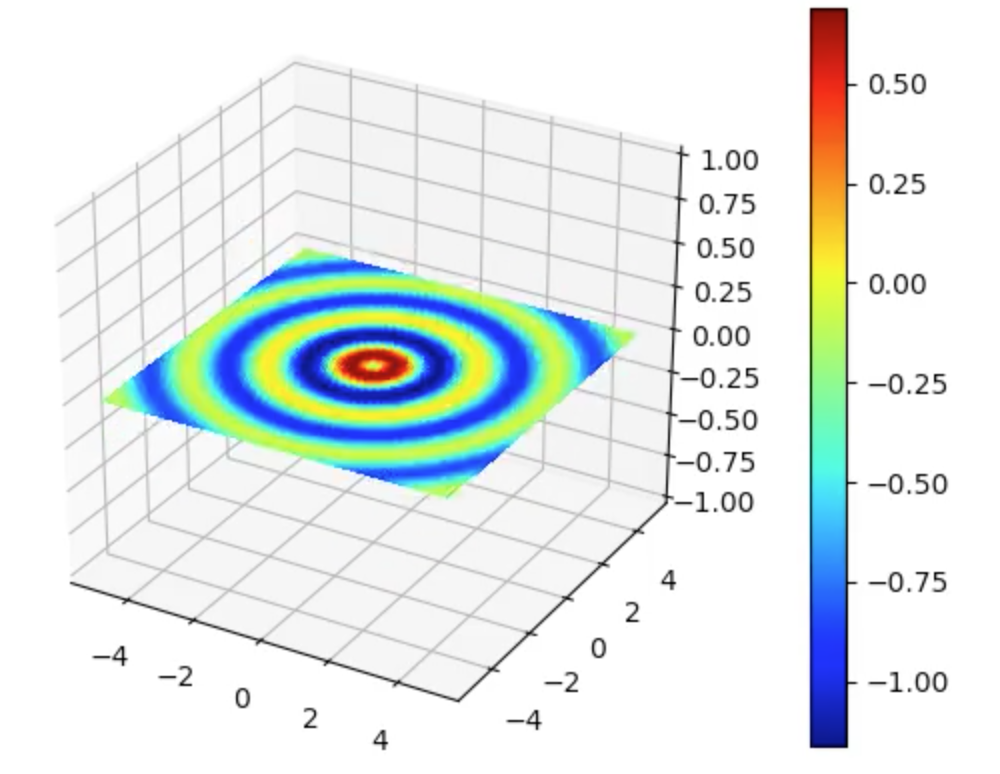
\includegraphics[width=\linewidth]{simulation/basich0.png}
        \caption{Wave motion at $h=0$}
    \end{subfigure}
    \begin{subfigure}{0.5\textwidth}
        \centering
        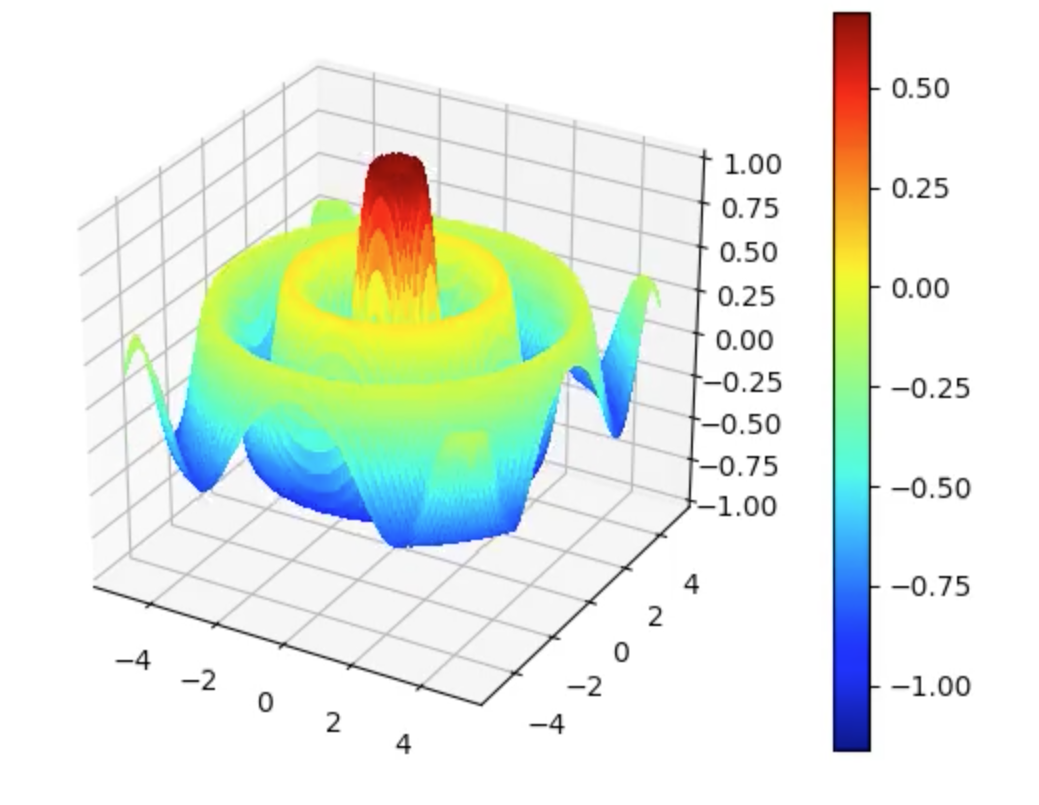
\includegraphics[width=\linewidth]{simulation/basichmax.png}
        \caption{Wave motion at $h=h_0$}
    \end{subfigure}
\caption{Simulation output generated with Python and Matplotlib. (a) represents the initial state of the wavefield, while (b) represents the state of the wave-field when the "droplet" at the centre is at its maximum height}
\label{fig:basicAnimation}
\end{figure}


\subsection{Constructing a GUI in Java}
Initially, a Java simulation was developed, which aimed to construct a pixel grid which could be used to represent a wave-field. Objects representing a given data point and a "frame" of these data points were constructed, and populated with amplitudes using (\ref{equ:basicHeight}). These amplitudes were then displayed in 2D by assigning them to an opacity scale, with 100\% opacity representing the maximum possible height and 100\% transparency representing the minimum possible height. For a 40,000 pixel frame running over 10 seconds, this process took approximately 9 seconds, but the animation process after this ran in real time. Figure \ref{fig:javaBasicHeight} shows a still image of this GUI taken when the "droplet" was at a minimum height of $-h_0$. This animation was a success, but at higher resolutions, latency when drawing the pixels to the screen caused it to lag, suggesting a need to either run multiple drawing tasks in parallel, or to display the droplet motion in an alternative way.

\begin{figure}
    \centering
    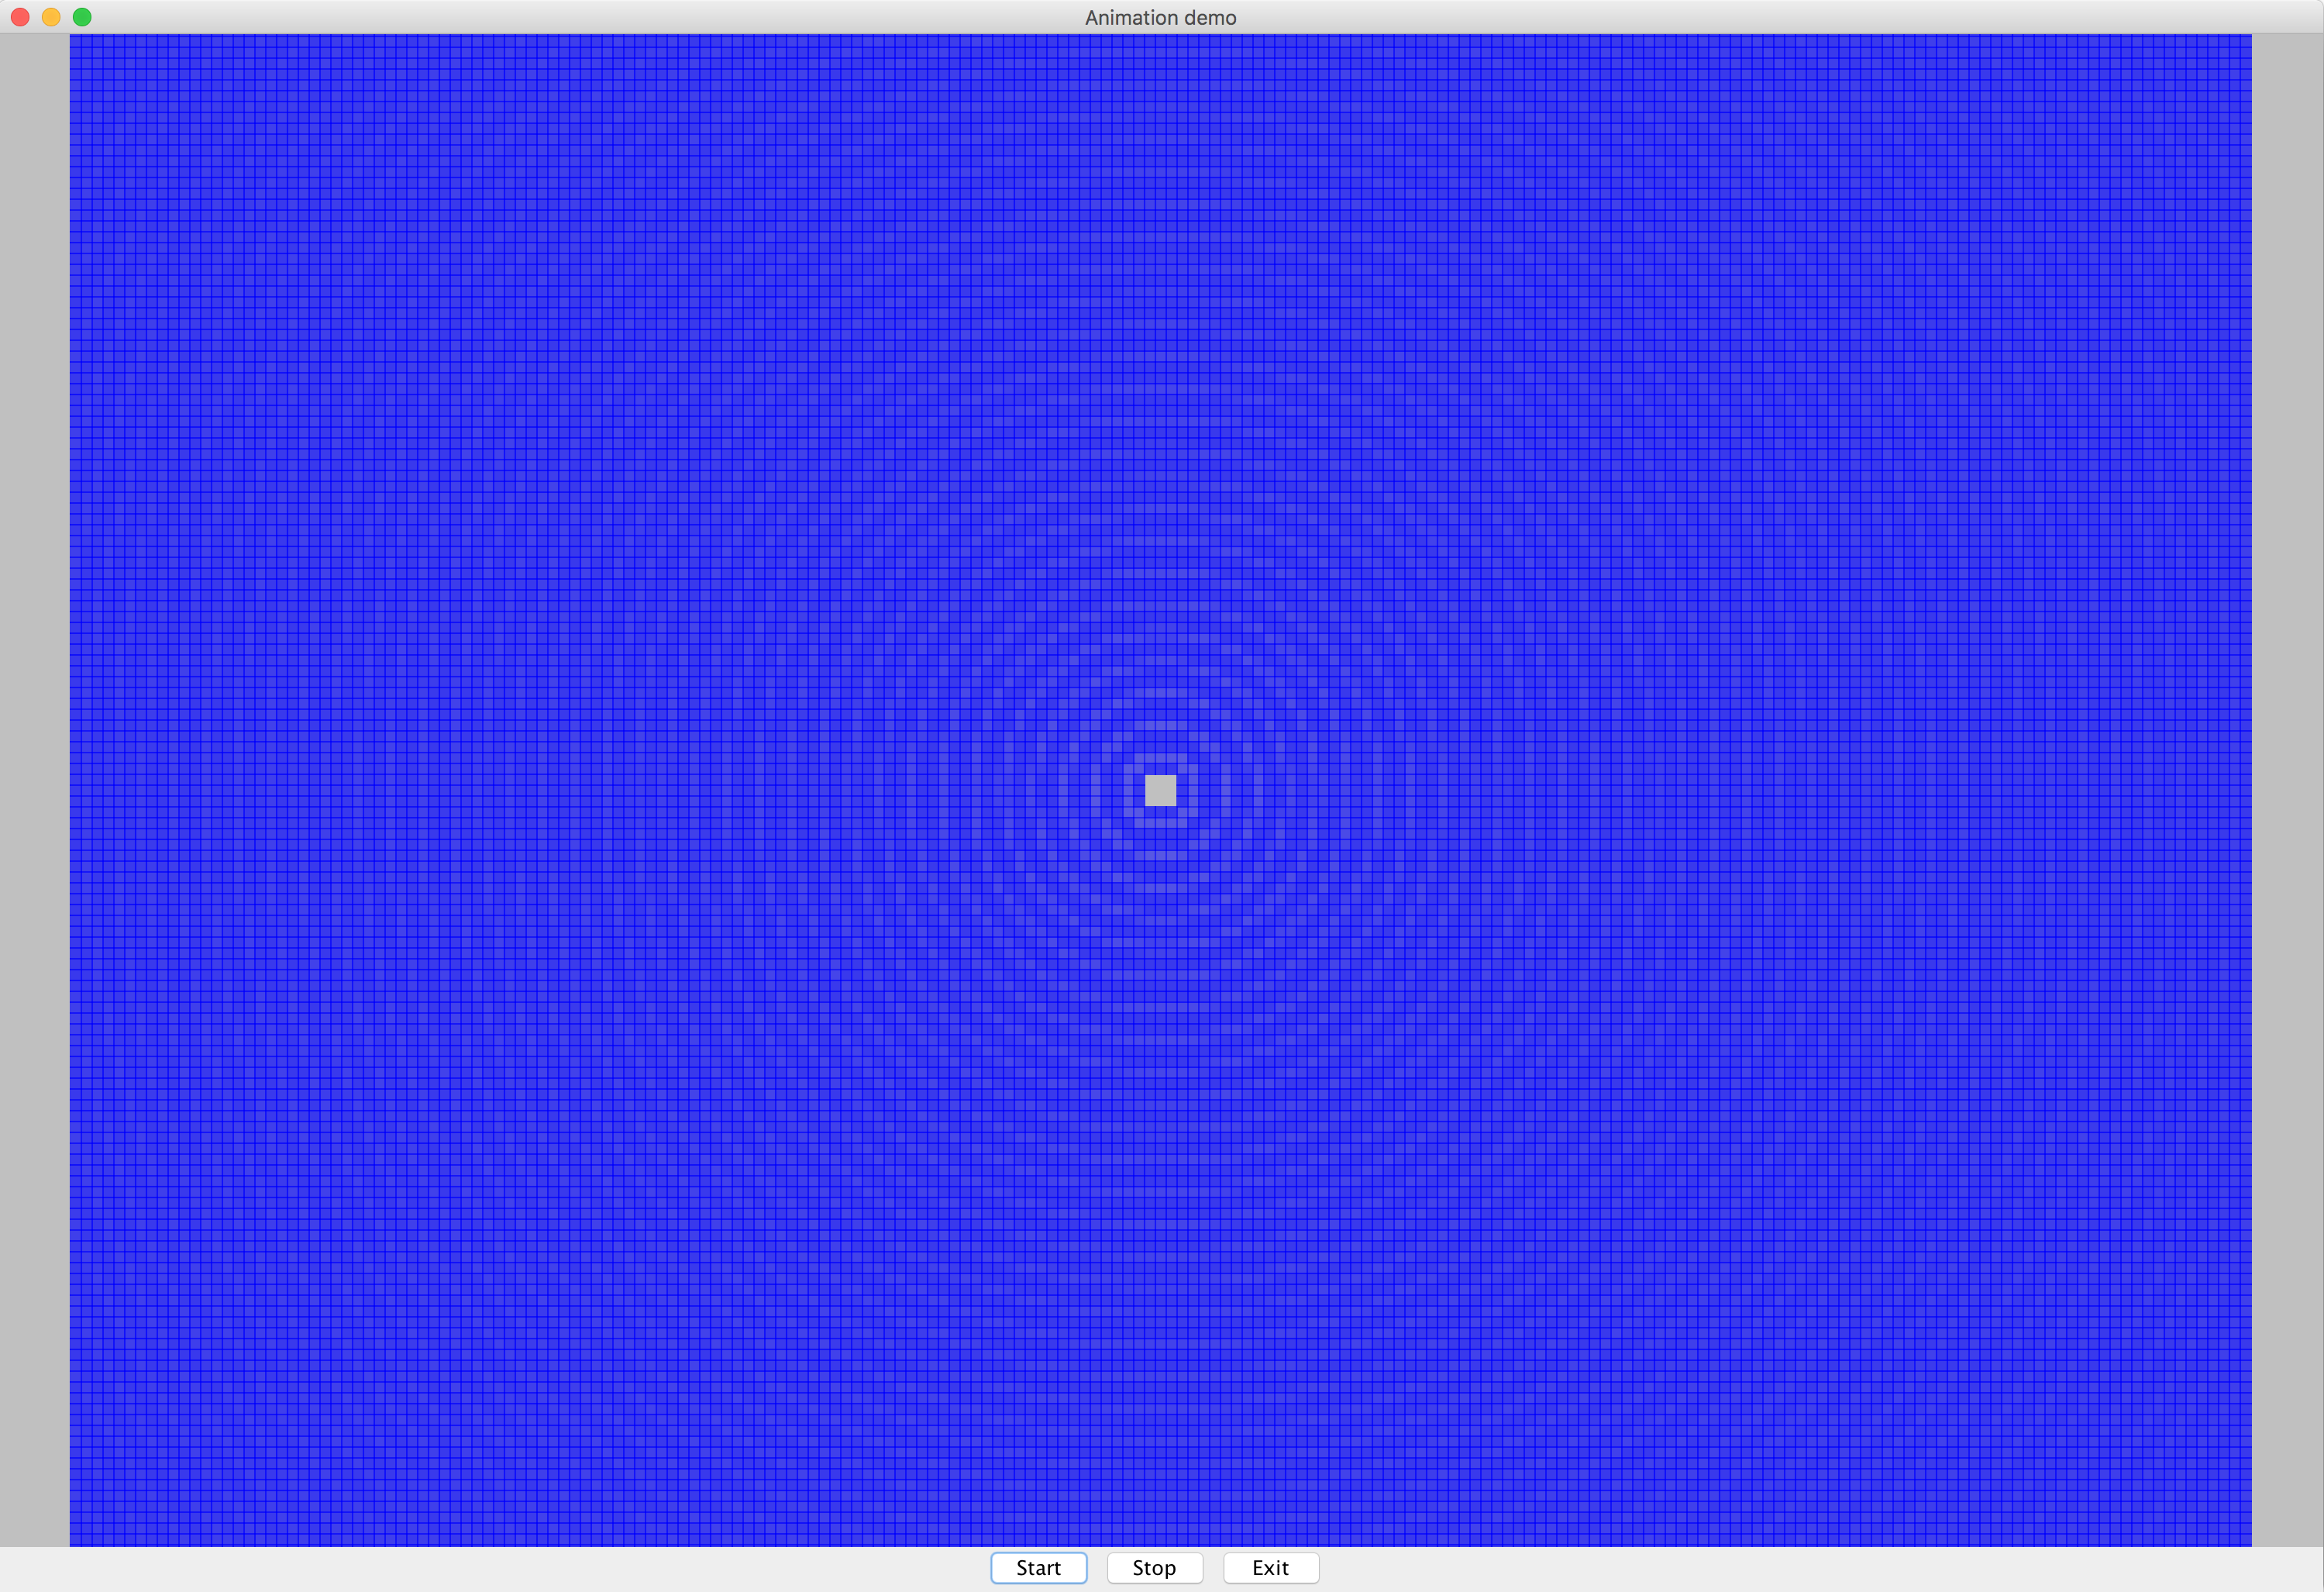
\includegraphics[width=\textwidth]{simulation/javaMaxHeight.png}
    \caption{A basic Java GUI, here showing the droplet at its minimum height of $-h_0$}
    \label{fig:javaBasicHeight}
\end{figure}

\subsection{Probabilistic prediction of position}
Having demonstrated the possibility of displaying wave-functions in Java, displaying an object representing a droplet was the next task. Here, the assumption was that the wave (described by Equation \ref{equ:probWaveEqn}) represented a probability density function. Therefore, for a given (and ideally infinitesimal) pixel n of area dA, the probability $P_n$ of finding the particle at pixel $n$ was calculated from that function. The height ($z_n$) of each pixel within that section was calculated, with ${P_n}/{z_n}$ representing the probability of the particle being at that pixel. The sum of probabilities for this section, $Z=\sum_n{P_n}$, defined the normalisation value of the thread. A random number generator then generated a number R such that $0\leq R \leq 1$, which was multiplied by $Z$ to give a relative random number. The program then looped back over all the pixels in the section, and repeatedly subtracts $P_n$ from $RZ$ until $RZ<0$. The first pixel where this condition is satisfied is determined to be the location of the droplet. This process could then be multi-threaded to improve computational efficiency.

The application of this to our project was that once the droplet is found at a given pixel, the distance between that pixel and the next pixel representing the location of the droplet is used to calculate the velocity v of the particle, assuming the droplet moves to the new pixel in the space of one period $T=1/f$. The wave-function was updated with the new velocity, once a Lorentz transform was accounted for. This whole process is repeated to find the trajectory of the pixel.

\begin{figure}
\centering
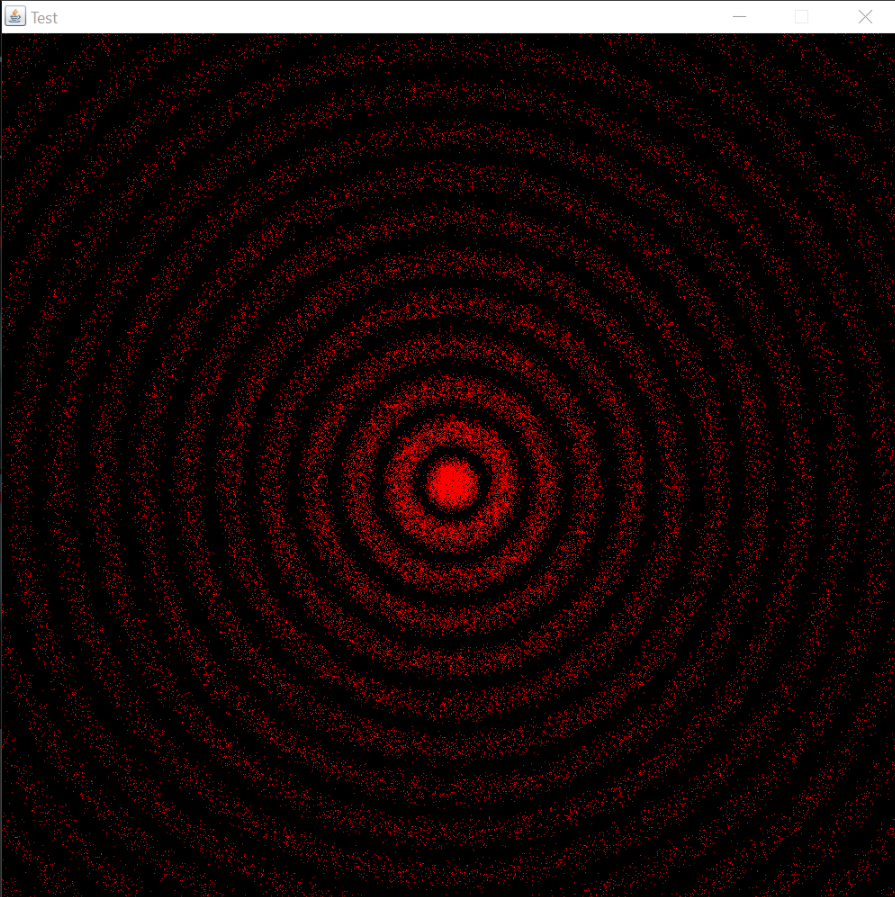
\includegraphics[width=\textwidth]{simulation/probabiltyPosition.png}
\caption{Results of the probabilistic prediction of the droplet position, where each dot represents the droplet being present at this point}
\label{fig:probabilisticPrediction}
\end{figure}

\begin{equation}
    h = -\cos(\omega t) J_0(\frac{\omega}{c} |\vec{r_f}-\vec{r_i}|)
    \label{equ:probWaveEqn}
\end{equation}

Although this process was successful, all it ended up proving was that a random position generator works. It does not accurately simulate the position of droplets created in our experiment. Therefore, we proceeded to calculate the equations of motion and the wave-function of the droplet at each point.

\todo{Finalise writeup of Matlab work}
\subsection{Rapid prototyping in Matlab}
In parallel to this, Matlab was chosen to test implementations of mathematical concepts found in our research, as it has a wide variety of built in libraries, such as for graphing software and advanced mathematical processes. Initially, equations of motion for the droplet were taken from \cite{oza2013trajectory}, where (\ref{equ:matlabPilotWave}) defines the wave-field of the particle and (\ref{equ:matlabWaveHeight}) defines the bath height over time. To implement these, a grid object was constructed and populated with x-y coordinates. A point in the middle of the grid was then selected as the starting position for a droplet, which was used as the centre of modelling for the first interaction.

\begin{equation}
m \vec{x}'' + D\vec{x}' + k\vec{x} = -mg\nabla h(\vec{x},t)
\label{equ:matlabPilotWave})
\end{equation}

\begin{equation}
h(\mathbf{x},t) = \sum_{n=-\infty}^{\floor{t/T_F}} A \mathbf{J}_0(k_F |\mathbf{x}-\mathbf{x}_p(nT_F)|) e^{-(t-nT_F)/(T_F M_e)}
\label{equ:matlabWaveHeight}
\end{equation}

Once a centre had been chosen, the wave-field generated by the droplet at that point was calculated at time $t=0$. Assuming that the droplet bounces in phase with the forcing frequency, the droplet next interacts with the bath at time $t=T_F$, where $T_F = 2/\omega$, with $\omega$ representing the forcing frequency of oscillation. The evolution of the wave-field during this time period was calculated from the Bessel function $\mathbf{J}_0$, and so the droplet experiences a (quasi-instantaneous) acceleration proportional to the gradient of the wave-field at the droplet's position. A new wave-field is calculated at the droplet's new position following this acceleration. This process is repeated, with the n most recent wave-fields added to the current wave-field, where n represents the number of threads used to calculate the wave-field. Each iteration of this process was represented with a frame in the animation, which contained a colour-coded $(x,y,z,t)$ point for the entire grid, as shown in Figure \ref{fig:matlabMaths}.

\begin{figure}
\centering
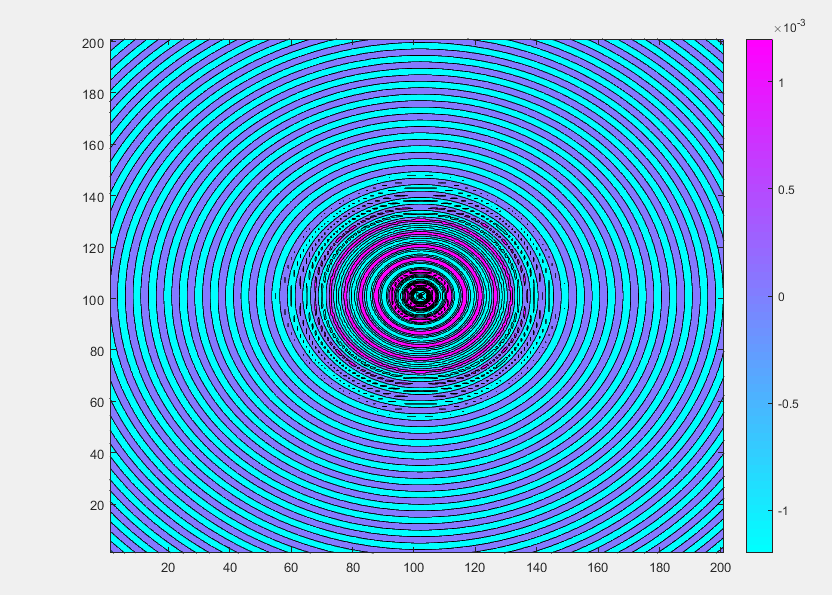
\includegraphics[width=\textwidth]{simulation/matlab.png}
\caption{The wave-field of a single droplet after multiple iterations, with a box size of 200x200 pixels and N=16. N was chosen as the machine used was capable of 8 threads and each impact� is calculated in parallel}
\label{fig:matlabMaths}
\end{figure}



\todo{AS to edit from here to end}

% Even with the fairly modest resolution and value of N used above frame generation was in the order of several minutes. With computational time scaling with the square of the simulation size, attempts at increasing the resolution would grow rapidly out of hand. However the most computationally intense process (accounting for around 90\% of script runtime with the above parameters) is the evolution of each impact’s wave field and this would scale with the ratio of N to number of threads on the machine being used and also would scale linearly with the number of droplets present in the simulation. While the limited resolution is arguably of low importance provided the results are accurate, the simulation time precluding the use of multiple droplets (3 droplets for example could take well over 15 minutes per frame) and limiting the value of N is far more detrimental to the simulation being capable of achieving valuable results.

In the physical situation the decay of each wave generated at an impact would be dependent only on the $Me$, parameter. (Eddi 2011, Information stored in faraday waves)  In numerical simulation only a limited number of wave can be stored within memory and dealt within in calculations but ideally the value of N should be chosen such that the contribution of an impact should be nearly negligible when it is removed from memory. However, due to computational limitations only the 16 most recent impacts were used in the calculation of the wave-field. 




% end AS edits

The issues encountered in terms of processing speed could be partially addressed by porting the mathematical model developed into Java.  While it was expected that this would enable more efficient  , the realistic improvement in speed that could be offered would not be able to entirely negate these problems.
It was clear at this point that, regardless of potential optimisation, the goal of having a interactive simulation was not within the scope of the project. It was subsequently  decided to focus on using the previously developed Java graphics system with the model prototype  within Matlab to create a number of pre-rendered videos with varying parameters.

\subsection{Using Java/matlab}

Due to calculation and graphical issues from Matlab and Java respectively, a possible solution was the execution of Java classes from a Matlab script. This would allow the calculations to be carried out in Java, outputted to a csv or text file and then read by the initial Matlab script for demonstration. This was implemented using the command() function in Matlab to navigate to the source folder, compile and then run the necessary classes. Due to time constraints, it was not possible to complete this. The main issue encountered was the use of external jar files (for bessel function) not allowing the java files to compile. Various solutions were attempted, however it would not work. It seemed better to move on when considering the lack of time and compilation problems.


\subsection{Theoretical motion of the particle}

Equations of motion for the droplet were taken from \cite{oza2013trajectory}, which showed that the surface wave produced on the $\textrm{n}^{\textrm{th}}$ impact of a particle at postion $r_n$ and time $T_n$ on a surface oscillating vertically at $\omega$ above the Faraday threshold is given by (\ref{equ:heightSurfaceWave}). Here, $ h(\vec{r} , t)$ is the height of the wave at $\vec{r}$, $J_0$ is a Bessel function of the first kind, and wave number $k$ satisfies the relation $ J_0 \left( k \vec{r_0} \right) = 0$. $\vec{r_0}$ is a numerical cutoff parameter, while the amplitude of the wave, A is material specific and determined by the system parameters used. The exponential decay term at the end of the equation describes the wave decaying over time at a rate determined by the memory $M_e$ and period of particle $T_f$.

\begin{equation}
h_n(\vec{r} , t) = A J_o\left(k\left|\vec{r} - \vec{r_n}\right| \right) e^{-\frac{\left(t-T_n\right)}{T_f M_e}}
\label{equ:heightSurfaceWave}
\end{equation}

The overall surface wave can thus be described by the sum of all waves produced by every prior impact. Assuming the particle only interacts with the surface once every period (when the particle is at its lowest point), the overall wave equation $h (\vec{x} , t)$ is thus given by (\ref{equ:heightSumSurfaceWaves}).

\begin{equation}
h(\vec{r} , t) = \sum_{n=-\infty}^{\frac{t}{T_f}} A J_o\left(k\left|\vec{r} - \vec{r_n}\right| \right) e^{-\frac{\left(t-n T_f\right)}{T_f\times M_e}}
\label{equ:heightSumSurfaceWaves}
\end{equation}

Furthermore, we know that the surface wave needs to consider relativistic effects. The coordinate transform on the wave formed by the $n^{\textrm{th}}$ impact of a particle at some velocity v is as follows:
\begin{equation}
h_n(\vec{r} , t) = A_0 cos\left(\omega_0 t - \frac{\gamma^2 \omega_0 v}{c^2}\right) J_0\left(k \left| \left(\vec{r} - \vec{r_n}\right)^{\prime \prime}  \right| \right)e^{-\frac{\left(t-n T_f\right)}{T_f\times Me}}
\end{equation}

Where:
\begin{equation}
\gamma = \frac{1}{\sqrt{1-\frac{v^2}{c^2}}}
\end{equation}
\begin{equation}
\left(\vec{r} - \vec{r_n}\right)^{\prime \prime} = \gamma^2(\vec{r_v}-\vec{v}t)+\gamma\vec{r_{\perp}}
\end{equation}

$\vec{r_v}$ and $\vec{r_{\perp}}$ are the components of $\left(\vec{r} - \vec{r_n}\right)$ in the direction of velocity and perpendicular to velocity respectively.

\subsection{Modelling assumptions and simulation mechanics}

The following assumptions were made during the simulation: 

\begin{enumerate}
\item The particle and surface waves produce are oscillating in phase.
\item The particle and surface only interacting within a small time frame, $T_i$ of the particles' lowest point.
\item Average force exerted by the particle over $T_i$ is given by an effective wave force $F_b$. $F_b$ depends on material parameters and the mass of the particle. It has a maximum magnitude equal to the weight of the particle.
\item The effect of the Lorentz transform is negligible.
\item Impulse applied to the particle in the vertical direction perpendicular to the surface is assumed to be negligible and the particle continues oscillating vertically at the same frequency and amplitude. 
\item Particle experiences no damping force
\item The overall wave equation $h(\vec{r} , t)$ is dominated by the waves due to the last $N$ bounces only. Waves formed longer than $N$ bounces ago are removed from the overall wave equation. This simplifies the computation of the infinite sum within the overall wave equation. In the java simulation, by integrating multi-threading methods into our calculation, we were able to efficiently perform calculations with $N = 300$.
\end{enumerate}

Following these modelling assumptions, the parameters of the system were set as follows \cite{Dotwave}:

\begin{itemize}
\item Particle mass, $m_p = 2.6\textrm{e}-7$ kg
\item Driving Frequency $\omega= 80$ Hz
\item Period of particle, $T_f = \frac{2}{\omega}$ s
\item Gravitational acceleration, $g = -9.81$ m/s
\item Effective force, $F_b = 1.3174e-6$ N
\item Wave number, $k = 1250$
\item Amplitude, A = $\frac{F_b}{m_pkg}$ m
\item N = 300
\end{itemize}

The simulation starts by initiating a number of droplets on the surface, which vertically oscillate and form waves. On impact, each wave is added to an ArrayList of 2-D waveforms. To determine the height at any point, the height of all waves at that location in the ArrayList was summed, according to the superposition principle.

From the assumptions made above, it can be shown that the change in velocity of the particle in the direction parallel to the surface is given by:
\begin{equation} \Delta \vec{v} = \frac{T_i  F_b}{m_p} \times \frac{dh(\vec{x} , t)}{d\vec{x}}\end{equation}
Where $m_p$ is the mass of the particle and the last term is the vector gradient of the wave.

In 1-D, the gradient at a point $x = x_0$ is given by:
\begin{equation} \frac{dy}{dx}\Bigr|_{x_0} = \lim_{x\to0} \frac{y(x+\delta x)-y(x-\delta x)}{2\delta x}\end{equation}

Using a Taylor expansion about $x_0$, it can be shown that for $\delta x\neq 0$:
\begin{equation} \frac{dy}{dx}\Bigr|_{x_0} = \frac{y(x+\delta x) - y(x-\delta x)}{2\delta x} - O(\delta x)\end{equation}
Where $O(\delta x)$ is the residual given by:
\begin{equation}O(\delta x) = \sum_{n=2}^{\infty} \left( \frac{y^{(n)}(x_0)}{n!\times (2\delta x)} \left[ \left( x+\delta x -x_0 \right)^n - \left(x-\delta x -x_0 \right)^n \right] \right)\end{equation}

The 2-D vector gradient of $h(\vec{r} , t)$ was determined by first finding the 1-D gradient in the x-direction by using $\delta \vec{r} = (\delta x,0)$, followed by that in the y-direction by using $\delta \vec{r} = (0,\delta y)$. The 1-D gradients in each direction corresponds to the component of the 2-D vector gradient in their respective directions. 

In our computational model, $|\delta \vec{r}| = 1\times 10^{-18}$ was used. The resolution of the Bessel functions used prevented the use of any value smaller than this. Attempts using $|\delta \vec{r}| = 1\times 10^{-19}$ resulted in gradients calculated to either have magnitude 0 or magnitude $\approx 30$, which does not match the shape of the first order Bessel function.

The wave velocity was calculated as $\approx 0.201$. The perturbation velocity was on the order of 0.001, corresponding to $\gamma = 1.00001$. For simplicity of simulation, the Lorentz effects were assumed to be negligible and left out of calculation.


\subsection{Simulation in the high- and low-memory regimes}

The goal of the first simulation was to show that walking occurs as a result of the high memory regime. The difference between the high memory and low memory regimes is the rate of decay of the waves created by each impact on the surface. In the high memory regime, the waves decay slowly, and so waves created in the distant past can still strongly influence the particle trajectory. However, in the low memory regime, the waves decay rapidly, so only waves created in the recent past can significantly influence the particle's trajectory.

To test this, two simulations were run, one at Me = 150 and one at Me = 15. In both simulations, N = 300 was used. The particle was allowed to first bounce on the spot to build up 300 waves in the overall wave equation, corresponding to t = 7.5s. The particle was then perturbed by spontaneously changing its velocity to $\vec{v} = (0.0005,0)$. The results of the high and the low memory regime simulations are shown in Figure \ref{fig:memory}.

\begin{figure}
	\centering
	\begin{subfigure}{\textwidth}
		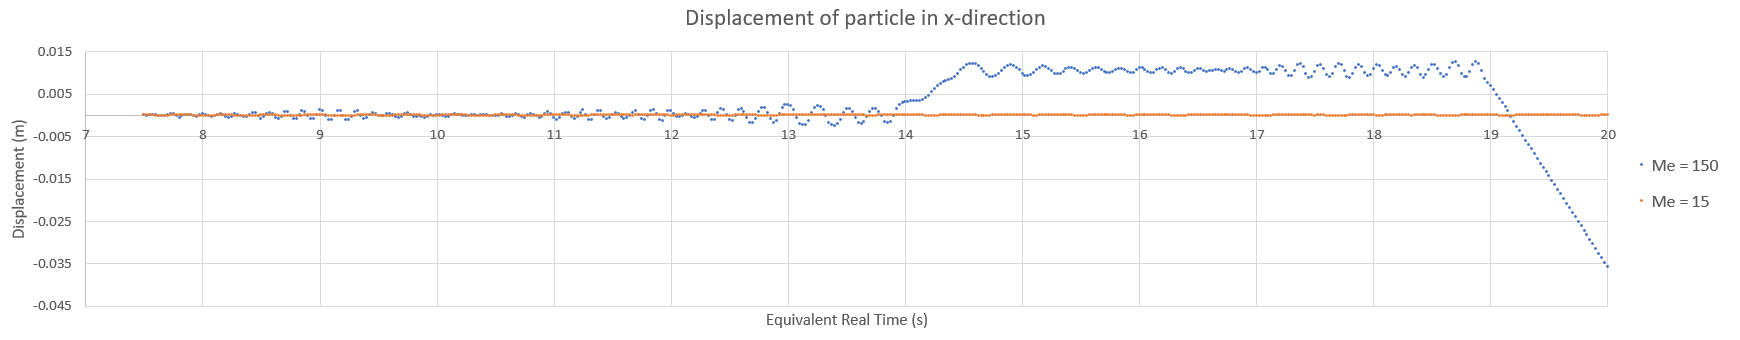
\includegraphics[width=\textwidth]{simulation/highmemory/displacement.png}
		\caption{Graph of displacement in the x-direction over time. $M_e=150$ represents the high memory regime, whereas $M_e=15$ represents the low memory regime}
		\label{fig:mem:displacement}
	\end{subfigure}
	
	\begin{subfigure}{\textwidth}
		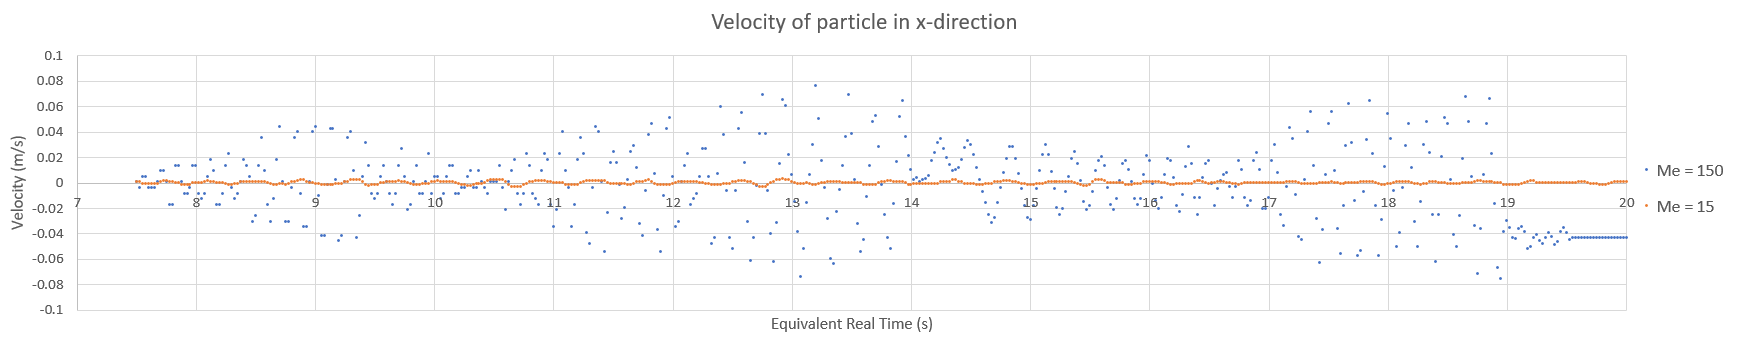
\includegraphics[width=\textwidth]{simulation/highmemory/velocity.png}
		\caption{In the high-memory regime, the particle velocity fluctuates chaotically before entering a stable state $\approx 11$s after perturbation. In the low-memory regime, the particle has negligible velocity}
		\label{fig:mem:velocity}.
	\end{subfigure}
	
	\begin{subfigure}{0.475\textwidth}
		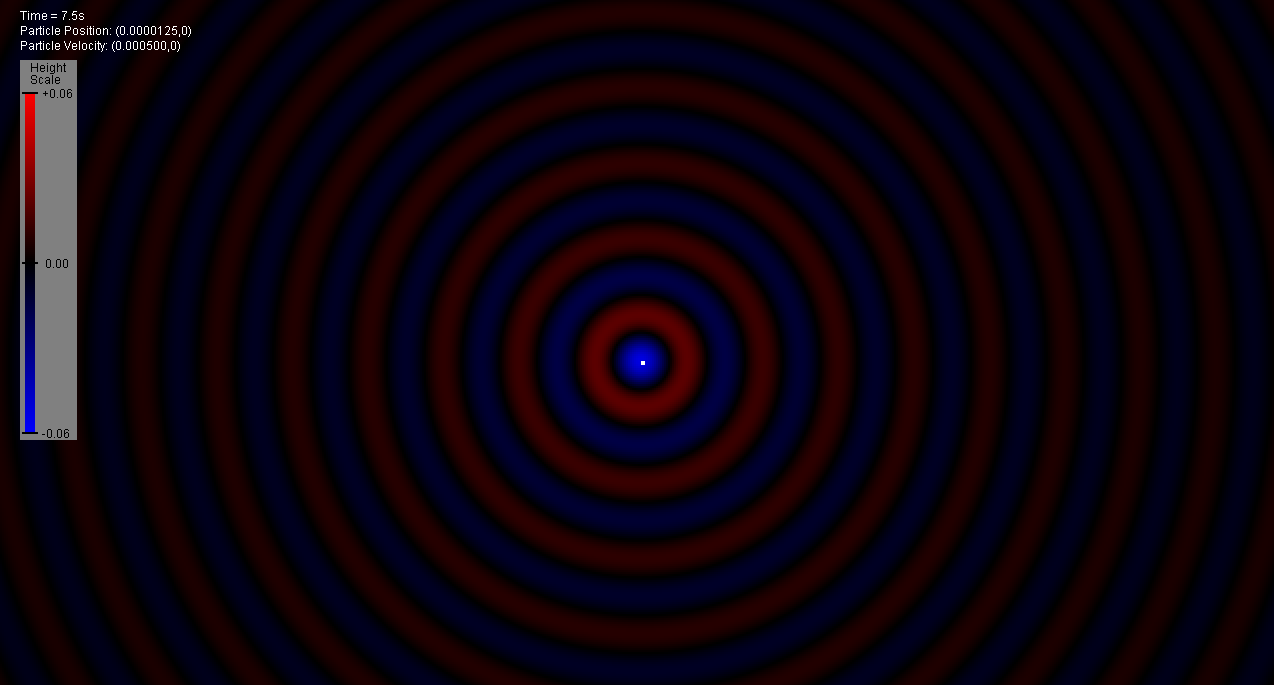
\includegraphics[width=\textwidth]{simulation/highmemory/wavefield75.png}
		\caption{The overall surface wave after $7.5$s; the wave-field has a similar shape to a 2-D harmonic potential well}
		\label{fig:mem:wavefield75}
	\end{subfigure}
	\hfill
	\begin{subfigure}{0.475\textwidth}
		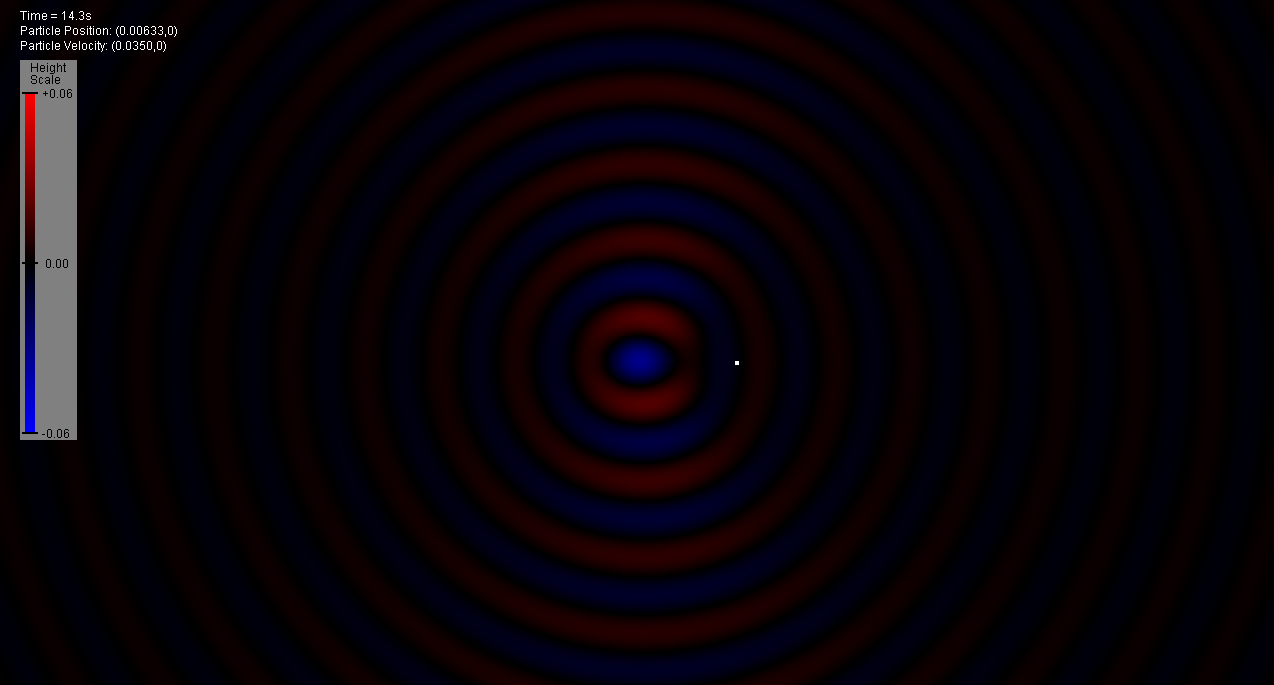
\includegraphics[width=\textwidth]{simulation/highmemory/wavefield145.png}
		\caption{The wave-field at $14.5$s, just prior to the particle breaking through the potential barrier and travelling}
		\label{fig:mem:wavefield145}
	\end{subfigure}
	
	\begin{subfigure}{0.475\textwidth}
		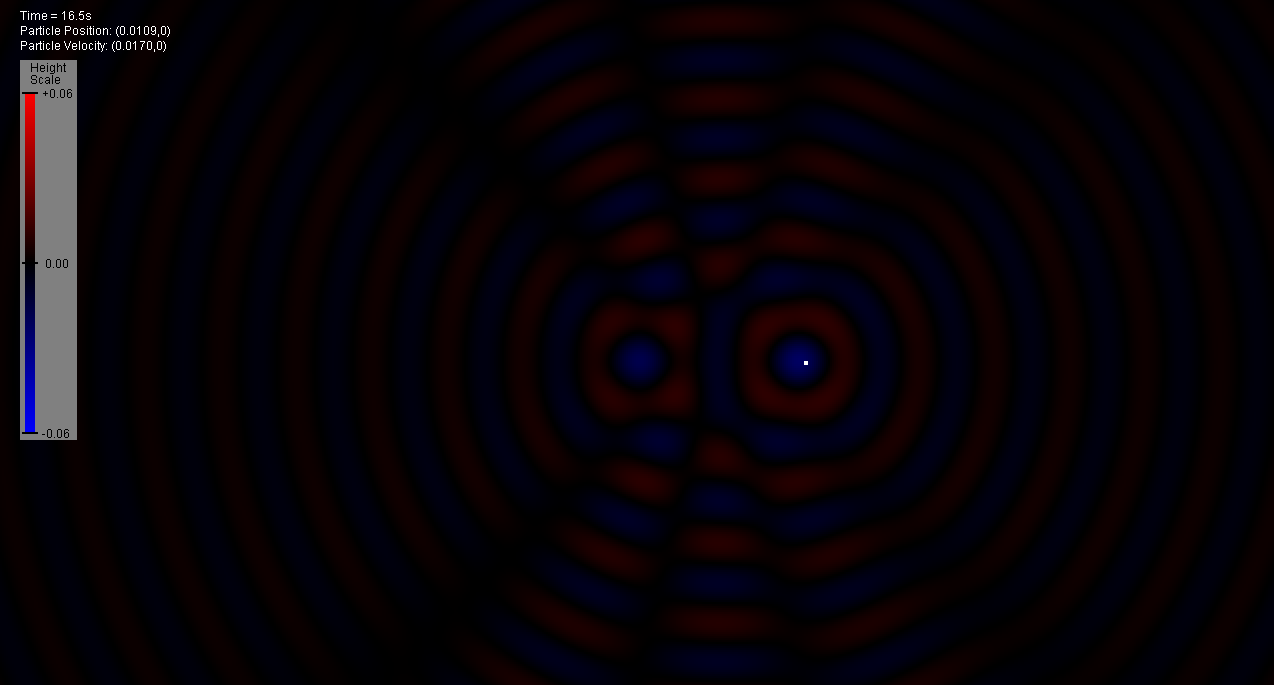
\includegraphics[width=\textwidth]{simulation/highmemory/wavefield165.png}
		\caption{Following multiple interactions with wave peaks, the particle decelerates and reforms a potential well}
		\label{fig:mem:wavefield165}
	\end{subfigure}
	\hfill
	\begin{subfigure}{0.475\textwidth}
		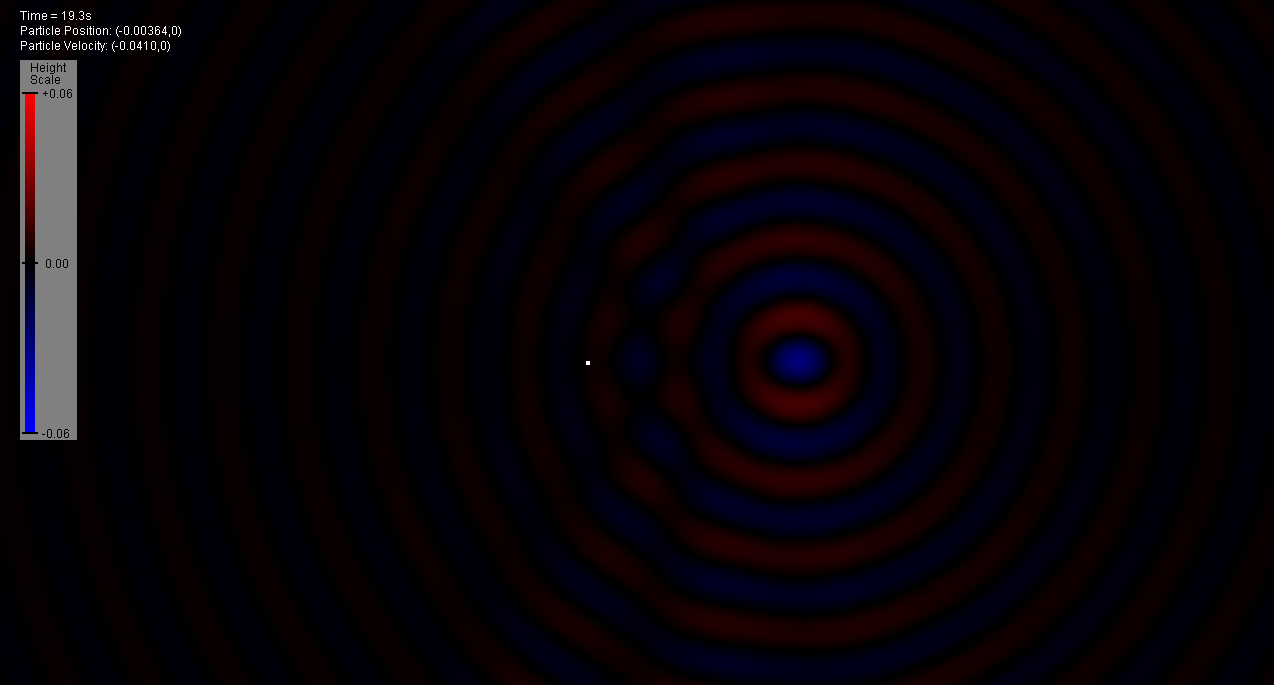
\includegraphics[width=\textwidth]{simulation/highmemory/wavefield195.png}
		\caption{The stable wave-field at $19.5$s, now displaced by $0.01m$.}
		\label{fig:mem:wavefield195}.
	\end{subfigure}
\caption{Results of the simulation in the high- and low-memory regime at different time periods}
\label{fig:memory} %actually includes low-memory regime as well
\end{figure}

We see from Figure \ref{fig:mem:velocity} that the particle velocity is chaotic. This causes the particle to oscillate around two centres of displacement, initially the start position, and later about the point $(0.01,0)$. We also observe in Figure \ref{fig:mem:wavefield75} that, prior to perturbation, the wave-field is similar in shape to a 2-D harmonic potential well, of width $\lambda/2$ and centred about the initial position of the particle. Upon perturbation, the particle oscillates, as expected for such a system. However, with each impact at positions away from the start position, new waveforms are added to the overall wave-function at these points. The waves formed at this point superpose over the 2-D harmonic potential well, flattening it along the x-axis. After approximately 7s, the peaks at $\lambda/2$ away from the start position along the x-axis were low enough that the particle could leave the well as shown in Figure \ref{fig:mem:wavefield145}.

The overall surface wave at 7.5s is shown in Figure \ref{fig:mem:wavefield75}. The wavefield is observed to be similar in shape to the 2-D harmonic potential well within half wavelength about the particles' start position. At this point, the particle is perturbed. As expected for a particle oscillating in a 2-D harmonic potential, the particle enters oscillatory motion. However, with each impact at positions away from the start position, new waveforms are added to the overall wavefunction at these points. The wave forms at this point superpose over the 2-D harmonic potential well flattening it along the x-axis. After approximately 7s, the peaks at half wavelength away from the start position along the x-axis were low enough that the particle could traverse it and leave the well about the start position. The overall surface wave at this point is shown in Figure \ref{fig:mem:wavefield145}. As the particle carries on in its trajectory away from the start position, it interacts with other smaller peaks causing it to slow down. As the particle slows down, the most recently formed waves are centered closer and closer together eventually reforming yet another potential well approximately about point (0.01,0). The overall surface wave at this point is shown in Figure \ref{fig:mem:wavefield165}. The particle then starts oscillating about this point for approximately 4s before the same mechanisms that allowed it to break through the first potential well occurs and the particle leaves the new formed well. Following this the particle enters a steady state and continues travelling with a stable velocity of (-0.043,0) $ms^{-1}$. The particle has thus started "walking".

The high memory regime simulation was repeated for perturbation velocity with magnitude between 0.0001 $ms^{-1}$ and 0.002 $ms^{-1}$ at intervals of 0.0001 $ms^{-1}$ to ensure that the above result of achieving walking was not due to specifically selected variables. In all cases the particle entered a steady "walking" state with velocities ranging form magnitude 0.00859 to 0.102. The final steady state velocities of each particle and their corresponding perturbation velocity can be found in Appendix \ref{steadystatevelocities}. No observable trend was found relating the steady "walking" state velocity and the perturbation velocity. \todo{need the steady state velocity list Gea}

The above results strongly suggest that a particle entering the walking state depends on $M_e$. Simulations were next conducted for $M_e$ between 15 and 150 at intervals of 0.1. Perturbation velocity was kept constant at (0.0005,0) $ms^{-1}$ in all simulations. The following conditions were set to determined if the particle has entered a walking state:

\begin{enumerate}
    \item $\Delta\vec{v} = 0$ for the past 20 time steps.
    \item The particle is at least 1 wavelength away from where it was initiated.
\end{enumerate}

If the particle in a simulation was detected to be in a walking state, the simulation would output the walking state velocity and the time at which "walking" was achieved. Each simulation was allowed to run for 10,000 time steps corresponding to 250s in real time. Any particle yet to achieve walking within this time frame was assumed to not be capable of entering the walking state. The results of these simulations can be found in Annex B. Visualisations of this data are shown as graphs in Figure \ref{fig:varmem}. 

As shown in Figure \ref{fig:varmem:walkingstate}, there is no clear threshold $M_e$ beyond which the particle will enter a walking state. From the plot it is observed that walking will not occur for Me < 50 but will occur for $M_e > 80$. The region in between, given by $50\leq M_e\leq80$, however, appears to be a grey area where whether a given Me leads to a walking state seems to follow some distribution. To determine the shape of this distribution a moving average of the previous 20 and next 20 points was plot against $M_e$. By observation, the plot here appears to be in the shape of a sigmoid curve. Using Origin Pro 2017s' non-linear curve fit function, the plot in was fitted to a Boltzmann sigmoid function with the top and bottom value fixed at 1 and 0 respectively. The Boltzmann sigmoid is given by:

\begin{equation}
y = (bottom) - \frac{(top)-(bottom)}{1+exp \frac{\left(x_0 - x \right)}{dx}}
\end{equation}

Where $x_0$ is the 50\% threshold found to be $64.54\pm0.04$.

The fit was found to have a R-squared value of 0.9974 and a reduced chi squared value of 5.33e-4 suggesting a decent fit. The plot of the residual of the fit against $M_e$, as shown in Figure \ref{fig:varmem:residualplot}, interestingly seems to be in the form of a wave packet. 

Figure \ref{fig:varmem:timewalking} shows the relation between time taken to enter the walking state and $M_e$. It is observed that the time taken has a wider spread for lower Me with a minimum that remains constant as Me increases. The minimum has a value of approximately $3\pm2$. This corresponds approximately to the time required to flatten the sides of the wave as described previously, thus allowing the particle to pass through it and leave the potential well around it.

The plot of the x-component of the walking velocity against $M_e$ is shown in Figure \ref{fig:varmem:walkingvel}. Since the particle was perturbed in the x-direction only, the y-component in all cases = 0. It is observed that approximately half of the simulations produced a walking velocity in the positive x-direction (the direction of perturbation), while the remaining half in the negative x-direction. 



\begin{figure}
	\centering
	\begin{subfigure}{\textwidth}
		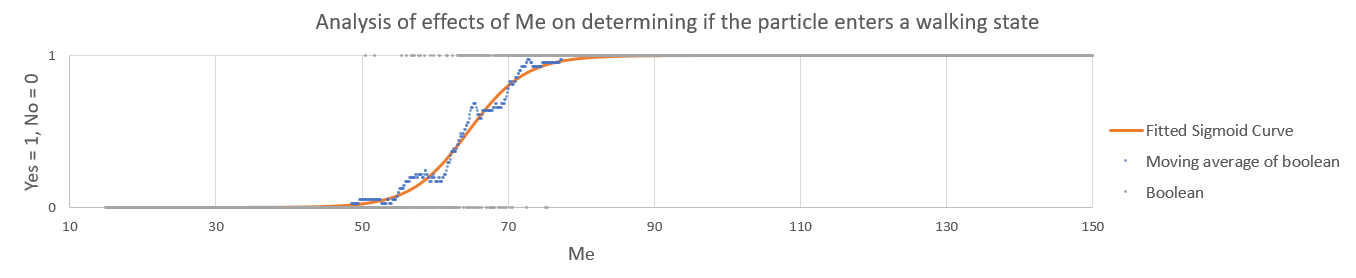
\includegraphics[width=\textwidth]{simulation/varmemory/walkingstate.png}
		\caption{Binary plot showing whether a particle was found to have entered a walking state within 10,000 time steps with 1 corresponding to yes and 0 to no against $M_e$. The moving average is plotted and fitted to a sigmoid curve}
		\label{fig:varmem:walkingstate}
	\end{subfigure}
	 \begin{subfigure}{\textwidth}
		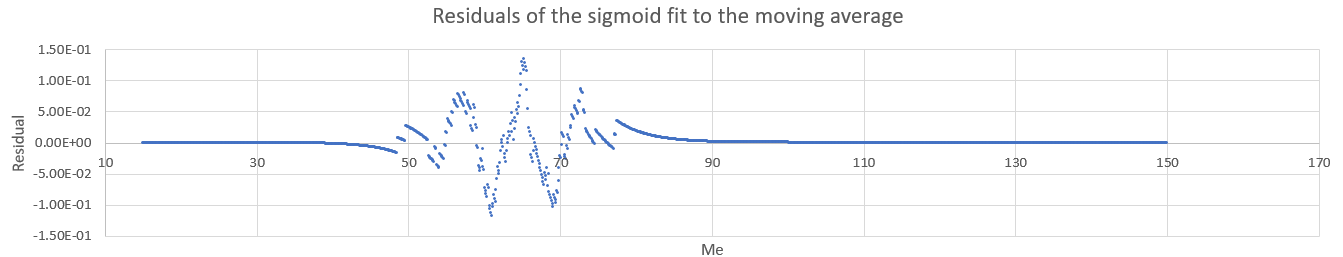
\includegraphics[width=\textwidth]{simulation/varmemory/residuals.png}
		\caption{Residual plot of the sigmoid fit of \ref{fig:varmem:walkingstate}}
		\label{fig:varmem:residualplot}
	\end{subfigure}
	\begin{subfigure}{\textwidth}
		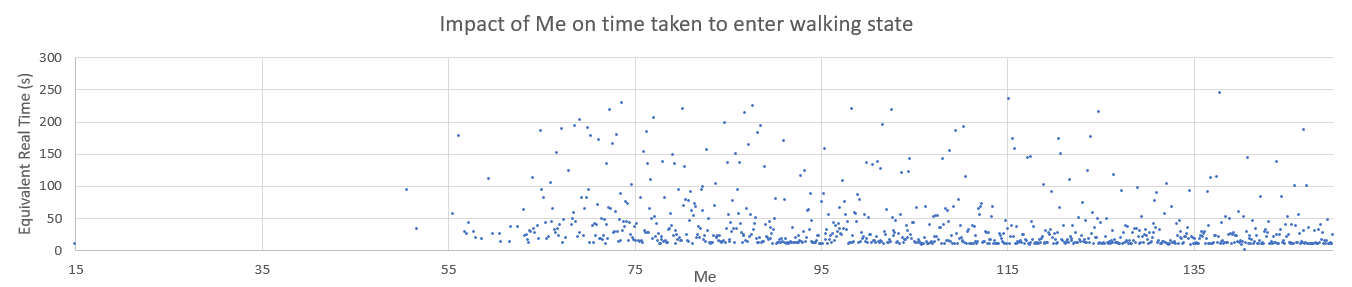
\includegraphics[width=\textwidth]{simulation/varmemory/meWalkingState.png}
		\caption{Plot of time taken for the particle to enter walking state against $M_e$ used in the simulation}
		\label{fig:varmem:timewalking}
	\end{subfigure}
	
	\begin{subfigure}{\textwidth}
		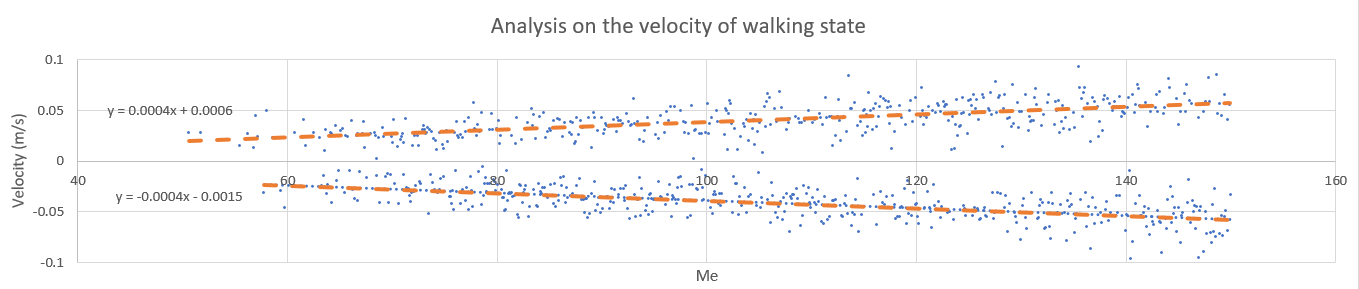
\includegraphics[width=\textwidth]{simulation/varmemory/velocityWalkingState.png}
		\caption{Plot of walking velocity of the particle against $M_e$ used in the simulation}
		\label{fig:varmem:walkingvel}
	\end{subfigure}
\caption{Analysis of the probability of a particle entering the walking state at different values of $M_e$}
\label{fig:varmem}
\end{figure}

\subsection{Conclusion}

The original aims of the simulation were to construct an interactive software package that could simulate and visualise the motion of droplets bouncing on a liquid surface. These aims were partially met: a non-interactive simulation was developed, whereby images from the software output could later be reconstructed into a video. However, due to computational limitations it was not possible to run this process in real time. This posed a significant barrier to the use of the simulation as a real-time educational aid, although the videos were still useful to illustrate the concepts to students in a classroom.

As work continued with the simulation, and the team developed a more detailed understanding of the theory behind droplet motion, additional goals were added to the project. This included determining the effect of changing simulation parameters such as the memory coefficient $M_e$, and allowing the end-user to vary those without needing to understand the source code. Again, these were partially met: detailed analysis of the effect of $M_e$ has been offered, an insight which would not be possible within the physical system. However, simulation parameters are still hard-coded, although this could change with relative ease in the future.

In order to extend the simulation further, such as by adding a parameter representing the in-elasticity of collisions between the droplet and the surface, or to implement boundary conditions, more nuanced mathematical models would be required. This meant that a subsidiary goal of representing quantum effects such as double-slit diffraction was not met. Implementing such boundary conditions, and correspondingly scaling up the computing power available, would therefore be a significant focus of future research in this area.